% Asset ID: AS2ForcesTikZ-004
% Source: MechYr2 Chapter 5 Friction PDF + Chapter 5/7 Forces Transcript
% Related lesson section: Worked Example 2
% Purpose: Show a box on a smooth horizontal floor pulled by 10N at 30 degrees.
\documentclass[tikz,border=8pt]{standalone}
\usepackage{amsmath}
\usetikzlibrary{arrows.meta, angles, quotes, decorations.pathmorphing}
\begin{document}
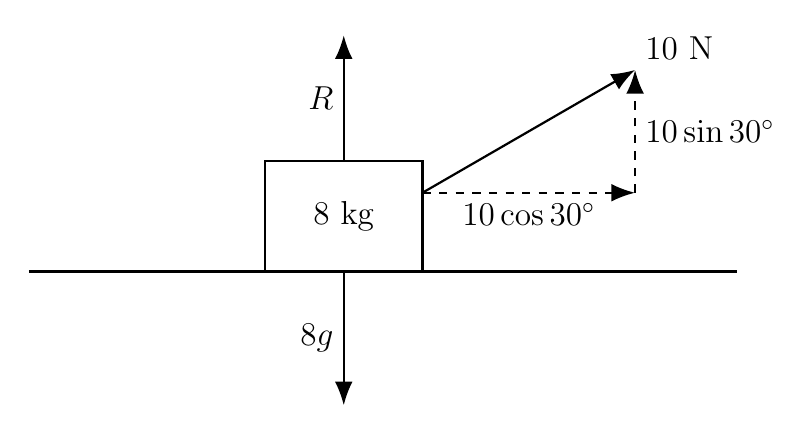
\begin{tikzpicture}[force/.style={-{Latex[length=3mm]}, thick}, comp/.style={-{Latex[length=3mm]}, thick, dashed}, label/.style={font=\large}, note/.style={font=\normalsize}]

\draw[thick] (-1,0)--(8,0); \draw[thick] (2,0) rectangle (4,1.4); \node[label] at (3,0.7) {$8\text{ kg}$};
\coordinate (A) at (4,1); \coordinate (B) at (6.7,2.56); \coordinate (C) at (6.7,1);
\draw[force] (A)--(B) node[above right,label] {$10\text{ N}$};
\draw[comp] (A)--(C) node[midway, below,label] {$10\cos30^\circ$};
\draw[comp] (C)--(B) node[midway, right,label] {$10\sin30^\circ$};
\draw[force] (3,1.4)--(3,3) node[midway,left,label] {$R$}; \draw[force] (3,0)--(3,-1.7) node[midway,left,label] {$8g$};
\end{tikzpicture}
\end{document}
